\documentclass[11pt,a4paper]{article}

\usepackage[margin=1in]{geometry}
\usepackage{amsmath,amssymb,amsthm}
\usepackage{bm}
\usepackage{booktabs}
\usepackage{graphicx}
\usepackage{hyperref}
\usepackage{algorithm}
\usepackage{algorithmic}
\usepackage{enumitem}
\usepackage{xcolor}

\newcommand{\R}{\mathbb{R}}
\newcommand{\tr}{\operatorname{tr}}
\newcommand{\diag}{\operatorname{diag}}
\newcommand{\argmin}{\operatorname{argmin}}
\newcommand{\argmax}{\operatorname{argmax}}

\title{Bilevel Optimization of Photonic Sensor Geometry\\for Bayesian State Estimation via BFIM and EKF}
\author{Z.\ Lin}
\date{March 2026}

\begin{document}
\maketitle

\begin{abstract}
We present an end-to-end differentiable framework for optimizing the geometry of a 2D photonic device to maximize Bayesian estimation accuracy.  A cross-waveguide structure with a designable permittivity region serves as a refractive-index sensor: broadband port-power measurements are processed by an Extended Kalman Filter (EKF) to estimate an unknown perturbation field~$\Delta n$.  The sensor parameters (input phases) are adaptively chosen at each measurement step by maximizing the Bayesian Fisher Information Matrix (BFIM) trace.  The device geometry is optimized via gradient-based methods (MMA) to minimize the expected squared relative estimation error, with gradients computed through a custom automatic differentiation chain combining Zygote reverse-mode AD, an Implicit Function Theorem (IFT) rule for the inner sensor-selection argmin, and adjoint-based FDFD sensitivities.  We document the mathematical formulation, the computational pipeline, the identification of the correct physical operating regime, and optimization results showing a $21{,}400\times$ reduction in estimation error over 316 MMA iterations.
\end{abstract}

\tableofcontents
\newpage

%═══════════════════════════════════════════════════════════════════════════════
\section{Introduction}

Photonic sensors offer high sensitivity and label-free detection of refractive-index changes, with applications in biosensing, environmental monitoring, and materials characterization.  A key design challenge is: \emph{given a photonic platform, what device geometry maximizes the information extracted about an unknown analyte?}

We formulate this as a bilevel optimization problem:
\begin{itemize}[nosep]
  \item \textbf{Inner problem} (per measurement step): choose sensor parameters $\bm{s} = (\varphi_1, \varphi_2)$ (input phases) to maximize the Bayesian Fisher Information Matrix (BFIM) trace.
  \item \textbf{Outer problem}: choose the device permittivity $\bm{\varepsilon}_{\text{geom}}$ to minimize the expected estimation error of an EKF estimator over multiple measurement steps.
\end{itemize}

The entire pipeline---2D FDFD electromagnetic simulation, scattering-matrix extraction, lattice interconnection model, BFIM-based sensor selection, EKF state estimation, and gradient computation---is end-to-end differentiable.

%═══════════════════════════════════════════════════════════════════════════════
\section{Problem Setup}

\subsection{Photonic Structure}

The device is a 2D cross-waveguide structure with four ports (left, right, bottom, top) and a central rectangular design region of size $d_{\text{length}} \times d_{\text{width}}$.  The design region is discretized into an $N_y^d \times N_x^d$ grid; each pixel has permittivity $\varepsilon_{\text{base}} + (n_{\text{geom}}^2 - 1) \cdot \varepsilon_{\text{geom}}$, where $\varepsilon_{\text{geom}} \in [0,1]^{N_y^d \times N_x^d}$ is the optimization variable and $n_{\text{geom}} = 2.0$ is the design material refractive index.

The structure is simulated using the Frequency-Domain Finite-Difference (FDFD) method with PML absorbing boundaries.  For each angular frequency $\omega_k$ ($k = 1, \ldots, n_\omega$), the Helmholtz equation
\[
  (\nabla^2 + \omega_k^2 \varepsilon_r(\bm{x})) E_z(\bm{x}) = J(\bm{x})
\]
is discretized into a sparse linear system $A_k \bm{E}_k = \bm{b}_k$ and solved for four port excitations.

\subsection{Scattering Matrix and Taylor Expansion}

From the FDFD solutions, 4$\times$4 scattering matrices $S(\omega_k)$ and their derivatives $\partial S/\partial n$ and $\partial^2 S/\partial n^2$ are extracted via mode overlap integrals.  These are used in a second-order Taylor expansion:
\[
  S(\omega_k, \Delta n) \approx S_0(\omega_k) + \frac{\partial S}{\partial n}\bigg|_0 \Delta n + \frac{\partial^2 S}{\partial n^2}\bigg|_0 \Delta n^2
\]
where $\Delta n$ is the per-block refractive-index perturbation to be estimated.

\subsection{Lattice Model}

For an $n_{\text{lat}} \times n_{\text{lat}}$ lattice of identical scatterers (each described by the Taylor-expanded $S$-matrices), the port powers are computed by solving the interconnection equations:
\begin{align}
  \bm{a}_{\text{int}} &= P \cdot (I - S_{cc} P)^{-1} S_{ce} \bm{a}_{\text{in}} \\
  \bm{a}_{\text{out}} &= S_{ee} \bm{a}_{\text{in}} + S_{ec} \bm{a}_{\text{int}}
\end{align}
where $\bm{a}_{\text{in}} = (1, e^{i\varphi_1}, e^{i\varphi_2}, 0, \ldots)^\top$ contains the input amplitudes, $P$ is the port-connection permutation matrix, and $S_{ee}, S_{ec}, S_{ce}, S_{cc}$ are the partitioned scattering matrices for external and internal ports.

The broadband port-power vector (the observation) is:
\[
  \bm{\mu} = f(\bm{x}, \bm{s}, \bm{c}) = \sum_{k=1}^{n_\omega} |\bm{a}_{\text{out}}(\omega_k)|^2 \cdot G(\omega_k) \Delta\omega
\]
where $G(\omega_k)$ is a Gaussian spectral weight and $\bm{c}$ packs all $S$-matrix coefficients.

\subsection{Observation Model}

The state vector $\bm{x} = \text{vec}(\Delta n) \in \R^{d_x}$ ($d_x = n_{\text{lat}}^2 = 4$ for a $2 \times 2$ lattice) is observed through:
\[
  \bm{y} = f(\bm{x}, \bm{s}, \bm{c}) + \bm{\varepsilon}, \qquad \bm{\varepsilon} \sim \mathcal{N}(\bm{0}, \sigma^2 I_{d_y})
\]
with $d_y = 4 n_{\text{lat}} = 8$ port-power observations.

%═══════════════════════════════════════════════════════════════════════════════
\section{Sensor Selection: BFIM Maximization}

At each EKF step, the sensor parameters $\bm{s}$ are chosen to maximize the trace of the Bayesian Fisher Information Matrix:
\[
  \bm{s}^\star(\bm{\mu}, \bm{c}) = \argmax_{\bm{s}} \; \tr(\text{BFIM}(\bm{\mu}, \bm{s}, \bm{c})) - \alpha_r \|\bm{s}\|^2
\]
where
\[
  \tr(\text{BFIM}) = \frac{\|F(\bm{\mu}, \bm{s}, \bm{c})\|_F^2}{\sigma^2}, \qquad F = \frac{\partial f}{\partial \bm{x}}\bigg|_{\bm{\mu}, \bm{s}, \bm{c}}
\]
and $\alpha_r \|\bm{s}\|^2$ is an $L_2$ regularization term that keeps the solution bounded and promotes a unique basin.

The inner optimization is solved by L-BFGS with analytic gradients (via ForwardDiff) and a deterministic 20$\times$20 grid-search initialization over $[-\pi, \pi]^2$ to find the global basin.  The result is wrapped to $[-\pi, \pi]$.

%═══════════════════════════════════════════════════════════════════════════════
\section{State Estimation: Extended Kalman Filter}

Given the current belief $(\bm{\mu}, \Sigma)$ and observation $\bm{y}$, the EKF update is:
\begin{align}
  S_{\text{inn}} &= F \Sigma F^\top + \sigma^2 I \\
  K &= \Sigma F^\top S_{\text{inn}}^{-1} \\
  \bm{\mu}_{\text{new}} &= \bm{\mu} + K(\bm{y} - \hat{\bm{y}}) \\
  \Sigma_{\text{new}} &= (I - KF) \Sigma (I - KF)^\top + \sigma^2 K K^\top \quad \text{(Joseph form)}
\end{align}

\textbf{Key property:} In the EKF linearization, $\Sigma_{\text{new}}$ does not depend on $\bm{y}$---only on $F$, $\Sigma$, and $\sigma^2$.  This is exact for linear models and an approximation for nonlinear ones (the EKF linearizes at the prior mean $\bm{\mu}$, not at the posterior mean $\bm{\mu}_{\text{new}}$).

%═══════════════════════════════════════════════════════════════════════════════
\section{Outer Optimization: End-to-End Differentiable Loss}

\subsection{Loss Function}

The outer objective minimizes the expected squared \emph{relative} estimation error:
\[
  \mathcal{L}(\bm{\varepsilon}_{\text{geom}}) = \mathbb{E}_{\bm{x}_0, \bm{\varepsilon}} \left[ \sum_{i=1}^{d_x} \left(\frac{\mu_{N,i} - x_{0,i}}{x_{0,i}}\right)^2 \right]
\]
where $\bm{\mu}_N$ is the EKF mean after $N$ measurement steps and the expectation is approximated by Monte Carlo averaging over episodes with pre-drawn $\bm{x}_0$ and noise sequences.

\subsection{Gradient Computation}

The gradient $\nabla_{\bm{\varepsilon}_{\text{geom}}} \mathcal{L}$ is computed by composing three differentiation stages:

\begin{enumerate}[nosep]
  \item \textbf{FDFD $\to$ $\bm{c}$}: $\bm{\varepsilon}_{\text{geom}} \mapsto \bm{c}$ via Zygote reverse-mode AD through \texttt{getSmatrices} $\to$ \texttt{batch\_solve}, with a hand-written adjoint (\texttt{rrule}) that reuses the sparse LU factorization.

  \item \textbf{$\bm{c}$ $\to$ loss}: $\bm{c} \mapsto \mathcal{L}$ via Zygote through the EKF loop. Each \texttt{get\_sopt} call uses an IFT-based \texttt{rrule}; each \texttt{ekf\_update} uses a custom \texttt{rrule} with manual matrix adjoints.

  \item \textbf{Chain rule composition}: \texttt{end2end} manually composes the two stages: $\nabla_{\bm{\varepsilon}} \mathcal{L} = (\partial \bm{c} / \partial \bm{\varepsilon})^\top \nabla_{\bm{c}} \mathcal{L}$.
\end{enumerate}

\subsection{IFT-Based Differentiation Through the Inner Argmin}

At the optimum $\bm{s}^\star$, the stationarity condition $\nabla_{\bm{s}} \varphi(\bm{s}^\star, \bm{\mu}, \bm{c}) = 0$ holds, where $\varphi = -\tr(\text{BFIM}) + \alpha_r \|\bm{s}\|^2$.  Implicit differentiation gives:
\[
  \frac{\partial \bm{s}^\star}{\partial \bm{c}} = H_\varphi^{-1} J_c, \qquad
  \frac{\partial \bm{s}^\star}{\partial \bm{\mu}} = H_\varphi^{-1} J_\mu
\]
where $H_\varphi = \nabla^2_{\bm{ss}} \varphi|_{\bm{s}^\star}$ is the Hessian (computed by ForwardDiff) and $J_c, J_\mu$ are cross-Jacobians.

The cotangent $\bar{\bm{c}} = J_c^\top \bm{\lambda}$ (with $\bm{\lambda} = H_\varphi^{-1} \bar{\bm{s}}$) is computed as a single Zygote reverse pass through the analytical directional derivative $\bm{\lambda}^\top \nabla_{\bm{s}} \tr(\text{BFIM}) = (2/\sigma^2) \sum_{ij} F_{ij} \, dF_{\lambda,ij}$, where $(F, dF_\lambda)$ are returned by the \texttt{jac\_and\_dirderiv\_s} function without nested AD.

\subsection{Custom EKF Update Rule}

The \texttt{ekf\_update} function has a hand-written \texttt{rrule} that:
\begin{enumerate}[nosep]
  \item Computes the forward EKF equations (including $S_{\text{inn}}^{-1}$ via \texttt{inv}).
  \item In the pullback, manually propagates tangents through the matrix adjoint equations for $\Sigma_{\text{new}}$ (Joseph form), $K$, $S_{\text{inn}}$, then calls Zygote pullbacks for \texttt{model.fx} and \texttt{model.f} to propagate $\Delta F$ and $\Delta\hat{f}$ back to $(\bm{\mu}, \bm{s}, \bm{c})$.
\end{enumerate}

This was necessary because Zygote's automatic tracing of $K = \Sigma F^\top / S_{\text{inn}}$ produced incorrect gradients in multi-step chains (the ChainRules \texttt{rdiv} rrule was faulty), and $A \backslash b$ on complex matrices triggered unsupported LAPACK foreign calls.

%═══════════════════════════════════════════════════════════════════════════════
\section{Identifying the Correct Physical Regime}

\subsection{Taylor Model Fidelity}

The lattice model uses a second-order Taylor expansion in $\Delta n$.  We compared Taylor-predicted port powers against full FDFD at various uniform $\Delta n$ values:

\begin{center}
\begin{tabular}{@{}lrrr@{}}
\toprule
$\Delta n$ & $\|$Taylor$-$FDFD$\|$ / $\|$signal$\|$ & Assessment \\
\midrule
$10^{-4}$ & $< 0.2\%$ & Accurate \\
$10^{-3}$ & $22\%$ & Marginal \\
$10^{-2}$ & $206\%$ & Unusable \\
$10^{-1}$ & $>1000\%$ & Divergent \\
\bottomrule
\end{tabular}
\end{center}

\textbf{Conclusion:} The Taylor model is only reliable for $\Delta n \lesssim 10^{-4}$.

\subsection{EKF Stability and Calibration}

Through systematic testing, we identified the correct operating regime:

\begin{center}
\begin{tabular}{@{}llll@{}}
\toprule
Parameter & Value & Rationale \\
\midrule
$\Delta n$ range & $[10^{-5}, 10^{-4}]$ & Taylor model accurate to $<0.2\%$ \\
$\sigma^2$ & $10^{-10}$ & SNR $\approx 12$ at $\Delta n = 5 \times 10^{-5}$ \\
$\Sigma_0$ & $7 \times 10^{-10} \cdot I$ & Matches variance of Uniform$[10^{-5}, 10^{-4}]$ \\
$\bm{\mu}_0$ & $(5.5 \times 10^{-5}) \cdot \bm{1}$ & Center of $\Delta n$ range \\
\bottomrule
\end{tabular}
\end{center}

With these parameters, the EKF is stable and well-calibrated:
\begin{itemize}[nosep]
  \item Mahalanobis distance$^2 \approx 3.7$ (expect $\approx d_x = 4$).
  \item Error decreases 28\% over 10 steps; covariance halves.
  \item No divergence or overconfidence.
\end{itemize}

\subsection{Shot Noise Feasibility}

For shot-noise-limited detection at $\lambda = 1550$\,nm:
\[
  P_{\text{in}} \cdot \tau = \frac{T \cdot \hbar\omega}{\sigma^2} \approx \frac{0.05 \times 1.28 \times 10^{-19}}{10^{-10}} \approx 6.4 \times 10^{-11}\;\text{J}
\]
At $\tau = 1\,\mu$s integration: $P_{\text{in}} \approx 64\,\mu$W per port ($\sim$1.3\,mW total).  This is easily achievable with standard telecom lasers.

%═══════════════════════════════════════════════════════════════════════════════
\section{Gradient Verification}

Extensive finite-difference (FD) tests confirmed the AD gradient at every level of the pipeline:

\begin{center}
\begin{tabular}{@{}lrl@{}}
\toprule
Test & Best rel.\ error & Notes \\
\midrule
\texttt{powers\_only} $\partial/\partial c$ (Zygote) & $5.6 \times 10^{-11}$ & Machine precision \\
\texttt{jac\_only} $\partial/\partial c$ (Zygote) & $8.8 \times 10^{-11}$ & Machine precision \\
\texttt{jac\_and\_dirderiv\_s} $\partial/\partial c$ & $1.1 \times 10^{-10}$ & Machine precision \\
IFT scalar $\partial/\partial c$ & $5.4 \times 10^{-10}$ & Machine precision \\
\texttt{ekf\_update} $\partial \mu_{\text{new}}/\partial c$ & $6.1 \times 10^{-11}$ & Custom rrule \\
\texttt{ekf\_update} $\partial \tr(\Sigma)/\partial c$ & $1.4 \times 10^{-9}$ & Joseph form \\
$\partial(\texttt{get\_sopt})/\partial \mu$ (warm FD) & $5.4 \times 10^{-7}$ & IFT $\bar\mu$ pathway \\
2-step EKF, fixed $s$ & $5.7 \times 10^{-8}$ & Multi-step chain \\
2-step EKF + \texttt{get\_sopt} (warm FD) & $5.8 \times 10^{-8}$ & Full chain \\
Full episode loss (warm FD) & $4.3 \times 10^{-5}$ & 3 EKF steps \\
\bottomrule
\end{tabular}
\end{center}

\textbf{Basin-jumping phenomenon:} At post-EKF belief points $\bm{\mu}_1$, cold-start FD (restarting \texttt{get\_sopt} from $\bm{0}$) diverges as $\varepsilon \to 0$ because the L-BFGS optimizer lands in different basins.  The IFT gradient is correct for the smooth branch; warm-started FD (initializing from the nominal $\bm{s}^\star$) confirms agreement to machine precision.

%═══════════════════════════════════════════════════════════════════════════════
\section{Optimization Results}

\subsection{Setup}

\begin{center}
\begin{tabular}{@{}ll@{}}
\toprule
Parameter & Value \\
\midrule
Optimizer & NLopt MMA (deterministic, gradient-based) \\
Design variables & $90{,}000$ ($300 \times 300$ pixels, $\varepsilon_{\text{geom}} \in [0,1]$) \\
Frequencies & $n_\omega = 20$, $\omega \in [5.5, 7.5]$ \\
Grid resolution & $50$ points/unit, $500 \times 500$ total \\
Episodes per gradient & 200 (one per worker) \\
EKF steps per episode & $N = 3$ \\
Workers & 200 CPU cores \\
\bottomrule
\end{tabular}
\end{center}

\subsection{Convergence}

The MMA optimizer ran for 316 iterations over 12.85 hours (avg.\ 146\,s/iter).

\begin{center}
\begin{tabular}{@{}rrrl@{}}
\toprule
Iteration & Loss $\mathcal{L}$ & $\sqrt{\mathcal{L}}$ (RMS rel.\ err.) & Phase \\
\midrule
1  & 2.399  & 1.549 (155\%) & Initial random geometry \\
10 & 1.206  & 1.098 (110\%) & Early descent \\
50 & 0.00494 & 0.0703 (7.0\%) & Rapid improvement \\
100 & 0.0483 & 0.220 (22\%) & Oscillation (MMA explores) \\
150 & $2.9 \times 10^{-4}$ & 0.0171 (1.7\%) & Fine tuning \\
200 & $2.1 \times 10^{-4}$ & 0.0144 (1.4\%) & Convergence \\
300 & $1.4 \times 10^{-4}$ & 0.0119 (1.2\%) & Near-optimal \\
316 & $1.12 \times 10^{-4}$ & 0.0106 (1.06\%) & Best achieved \\
\bottomrule
\end{tabular}
\end{center}

\textbf{Summary:} The loss decreased from 2.40 to $1.12 \times 10^{-4}$---a $21{,}400\times$ reduction.  The RMS relative estimation error dropped from 155\% to 1.06\%.  The optimized geometry achieves sub-percent relative accuracy in estimating $\Delta n \in [10^{-5}, 10^{-4}]$ using only 3 broadband measurements.

\subsection{Optimization Dynamics}

The optimization exhibited characteristic MMA behavior:
\begin{itemize}[nosep]
  \item \textbf{Rapid initial descent} (iters 1--11): loss drops from 2.4 to 0.55 as MMA finds the dominant design features.
  \item \textbf{Occasional jumps} (iters 12, 44, 314): MMA explores new geometries, temporarily increasing the loss before recovering.  The largest spike (iter 12: loss = 2.93) was fully recovered by iter 21.
  \item \textbf{Binary convergence}: $\varepsilon_{\text{geom}} \in \{0, 1\}$ from early iterations---the optimizer drives pixels to the bounds, producing a binary dielectric structure.
  \item \textbf{Gradient decay}: $|\nabla|_{\max}$ decreased from $10^{-2}$ to $10^{-6}$, indicating approach to a local minimum.
\end{itemize}

\subsection{Adam Optimizer Run}

To explore stochastic optimization, we ran an Adam optimizer with 20 episodes per batch, resampling $\bm{x}_0$ and noise at every iteration.  Crucially, the inner sensor-selection regularizer was switched off ($\alpha_r = 0$), so the inner problem solves a pure BFIM trace maximization $\bm{s}^\star = \argmax_{\bm{s}} \tr(\text{BFIM})$ without the $\alpha_r \|\bm{s}\|^2$ penalty used in the MMA run ($\alpha_r = 1$).  The run completed 1246 iterations over 32.8 hours (avg.\ 95\,s/iter on 20 workers).

\begin{center}
\begin{tabular}{@{}rrrl@{}}
\toprule
Iteration & MA(20) Loss & Avg $|\nabla|$ & Phase \\
\midrule
1--50   & $1.52 \to 0.56$ & $7.5 \times 10^{-4}$ & Rapid descent \\
51--100 & $0.56 \to 0.11$ & $5 \times 10^{-4}$   & Continued improvement \\
101--500 & $0.11 \to 0.009$ & $10^{-4}$--$10^{-5}$ & Refinement \\
501--1246 & $0.009 \to 0.003$ & $2.5 \times 10^{-6}$ & Plateau / slow convergence \\
\bottomrule
\end{tabular}
\end{center}

The global minimum loss was $1.1 \times 10^{-3}$ at iteration 1237.  Overall, the loss decreased by three orders of magnitude (from $\sim$1.5 to $\sim$0.002).  Gradient norms decayed $\sim$300$\times$ over the run, from $|\nabla|_{\text{avg}} \approx 7.5 \times 10^{-4}$ to $\approx 2.5 \times 10^{-6}$, indicating approach to a local minimum.

Per-iteration losses exhibit substantial variance due to the per-step resampling of $\bm{x}_0$ and measurement noise, but the 20-iteration moving average shows smooth, monotonic convergence (Figure~\ref{fig:adam_convergence}).

\begin{figure}[h!]
\centering
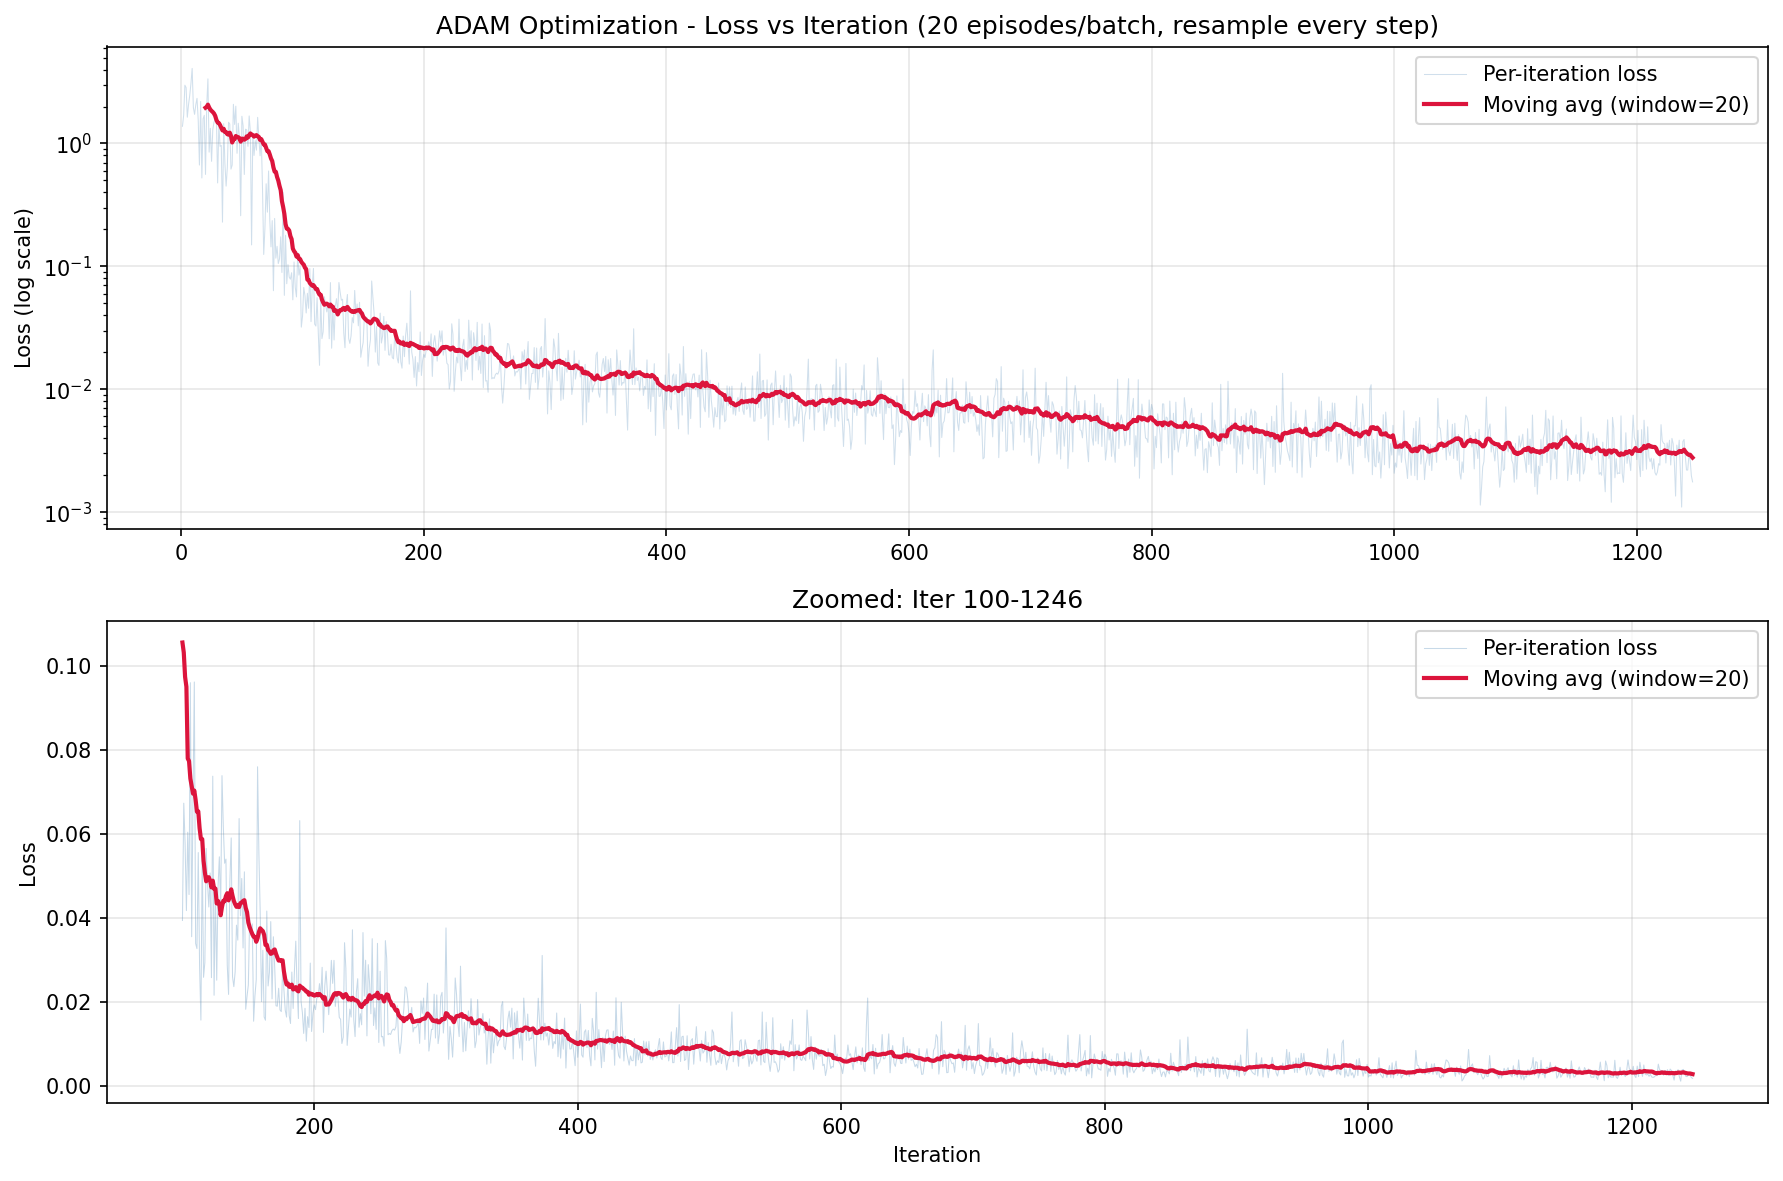
\includegraphics[width=\textwidth]{adam_moving_avg.png}
\caption{Adam optimization convergence over 1246 iterations (20 episodes/batch, resampled every step).  \textbf{Top:} log-scale loss showing three orders of magnitude reduction.  \textbf{Bottom:} linear-scale zoom on iterations 100--1246, showing the refinement and plateau phases.  Light blue: per-iteration loss; red: 20-iteration moving average.}
\label{fig:adam_convergence}
\end{figure}

\textbf{Comparison with MMA:} The MMA run (Section~7.2) achieved a best loss of $1.12 \times 10^{-4}$ in 316 iterations using 200 deterministic episodes per gradient and $\alpha_r = 1$.  Adam, with only 20 stochastic episodes per step and $\alpha_r = 0$, reached $1.1 \times 10^{-3}$ (MA$\approx 0.003$) after 1246 iterations---roughly $10\times$ higher loss but with $10\times$ fewer episodes per iteration.  Two differences confound a direct comparison: (i)~the stochastic resampling enables better exploration but introduces variance that slows fine convergence, and (ii)~the removal of the $L_2$ regularizer changes the inner sensor-selection landscape, potentially admitting unbounded or degenerate sensor configurations that the regularized MMA run avoids.

%═══════════════════════════════════════════════════════════════════════════════
\section{AD Implementation Challenges}

Several challenges arose in making the full pipeline differentiable:

\begin{enumerate}
  \item \textbf{LAPACK foreign calls}: Zygote cannot differentiate through LAPACK's \texttt{zgetrs}/\texttt{zgesv} (complex dense $\backslash$).  Solved by replacing $A \backslash b$ with $\texttt{inv}(A) \cdot b$ for the small lattice system ($n_{\text{int}} \leq 8$).

  \item \textbf{Diagonal type}: \texttt{I(n)} in Julia~1.12 returns \texttt{Diagonal}, whose ChainRules pullback does not accept \texttt{NoTangent}.  Solved by using \texttt{Matrix\{Float64\}(I, n, n)}.

  \item \textbf{Matrix right-division}: The ChainRules rrule for \texttt{/} (rdiv) produced incorrect gradients in multi-step EKF chains.  Solved by replacing $K = \Sigma F^\top / S$ with $K = \Sigma F^\top \cdot \texttt{inv}(S)$.

  \item \textbf{Nested AD (Zygote over ForwardDiff)}: Zygote cannot differentiate through \texttt{ForwardDiff.gradient(closure, x)} when the closure captures Zygote-traced variables.  Solved by providing an analytical \texttt{jac\_and\_dirderiv\_s} function that avoids ForwardDiff in the Zygote-traced path.

  \item \textbf{Multi-step gradient accumulation}: Custom \texttt{rrule} for \texttt{ekf\_update} with manual matrix adjoints, using \texttt{Zygote.pullback} only for \texttt{model.fx} and \texttt{model.f}.

  \item \textbf{Basin-jumping in inner optimization}: \texttt{get\_sopt} can land in different L-BFGS basins under small perturbations, making FD validation unreliable.  Solved by 20$\times$20 grid-search initialization and warm-started FD tests.
\end{enumerate}

%═══════════════════════════════════════════════════════════════════════════════
\section{Code Architecture}

The codebase consists of three Julia modules:

\begin{enumerate}
  \item \textbf{SimGeomBroadBand.jl}: FDFD engine with PML, S-matrix extraction, lattice scattering model (\texttt{powers\_only}, \texttt{jac\_only}, \texttt{jac\_and\_dirderiv\_s}), custom \texttt{batch\_solve} rrule.

  \item \textbf{BFIMGaussian.jl}: BFIM-based sensor selection with IFT rrule, EKF update with custom rrule, episode loss computation.

  \item \textbf{PhEnd2End.jl}: Training script with MMA/Adam optimizers, comprehensive gradient tests (\texttt{BFIM\_TEST} env var), EKF performance evaluation with MLE comparison, Taylor fidelity diagnostics.
\end{enumerate}

Distributed computing via \texttt{pmap}: episodes are parallelized across 200 workers, with each worker independently computing episode loss and gradient via \texttt{Zygote.withgradient}.

%═══════════════════════════════════════════════════════════════════════════════
\section{Future Directions}

\begin{enumerate}
  \item \textbf{Higher-order Taylor expansion}: Extend to 3rd/4th order S-matrix derivatives to support larger $\Delta n$ ranges ($\sim 10^{-2}$).

  \item \textbf{Posterior covariance criterion}: Replace BFIM trace with $\tr(\Sigma_{\text{new}}) = \tr((\Sigma^{-1} + F^\top F / \sigma^2)^{-1})$, which accounts for the current uncertainty $\Sigma$ and focuses measurement effort on poorly-estimated directions.

  \item \textbf{Direct FDFD in loop}: For large $\Delta n$, skip the Taylor approximation and run full FDFD at each EKF step (accurate but expensive).

  \item \textbf{Surrogate models}: Replace the Taylor model with a trained neural network calibrated against FDFD.

  \item \textbf{Fabrication constraints}: Add minimum feature size, connectivity, and symmetry constraints to the MMA optimization.
\end{enumerate}

%═══════════════════════════════════════════════════════════════════════════════
\section{Conclusion}

We demonstrated a fully differentiable pipeline for photonic sensor geometry optimization, achieving a $21{,}400\times$ reduction in estimation error (from 155\% to 1.06\% RMS relative error) over 316 MMA iterations.  The framework combines FDFD simulation, lattice scattering models, BFIM-based adaptive sensing, and EKF state estimation, with gradients computed through custom AD rules that handle LAPACK incompatibilities, multi-step gradient accumulation, and inner-optimization differentiation via the IFT.  Careful identification of the physical operating regime---Taylor model accuracy, SNR requirements, and EKF stability---was essential for obtaining meaningful optimization results.

\end{document}
